The clock of a computer or a watch counts the oscillations of a quartz crystal. The crystal behaves like a series circuit of $L_1$, $C_1$ and $R_1$, from its elastic vibration, in parallel with the capacitance $C_0 = \CzO$ of its electrodes. The graph shows its measured impedance (logarithmic axis) near the series resonance at $f_s = \fsO$; the horizontal axis shows the distance $f - f_s$ from it.

\begin{center}
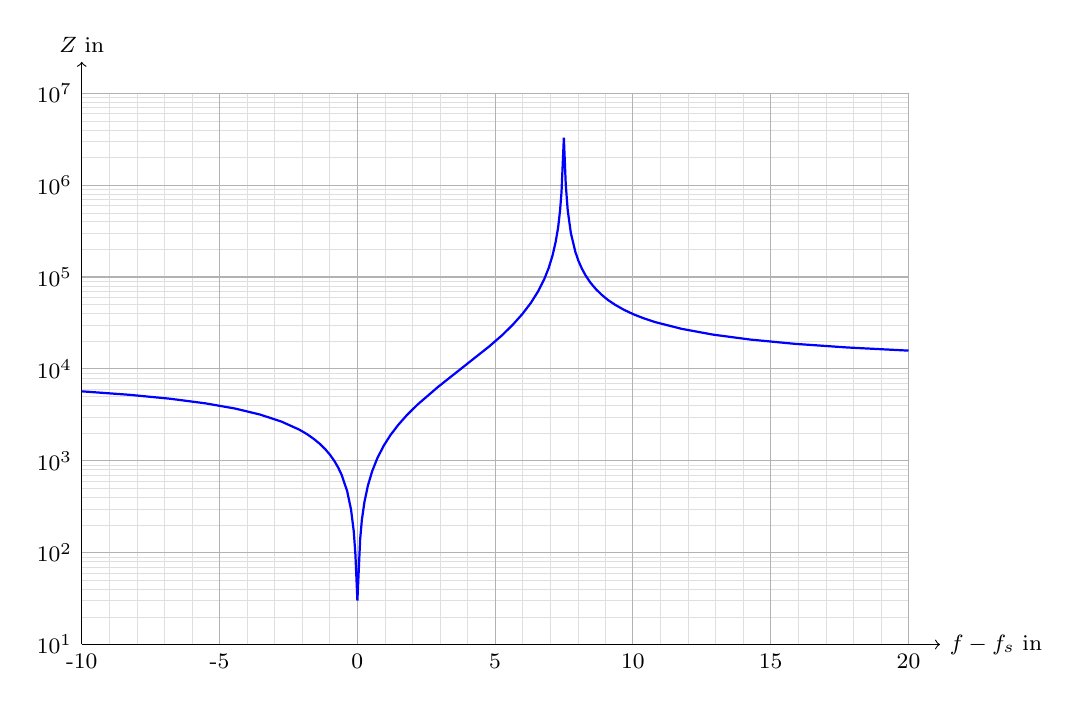
\begin{tikzpicture}[font=\footnotesize]
 \draw[gray!25, very thin] (0.350,0) -- (0.350,7.000) (0.700,0) -- (0.700,7.000) (1.050,0) -- (1.050,7.000) (1.400,0) -- (1.400,7.000) (2.100,0) -- (2.100,7.000) (2.450,0) -- (2.450,7.000) (2.800,0) -- (2.800,7.000) (3.150,0) -- (3.150,7.000) (3.850,0) -- (3.850,7.000) (4.200,0) -- (4.200,7.000) (4.550,0) -- (4.550,7.000) (4.900,0) -- (4.900,7.000) (5.600,0) -- (5.600,7.000) (5.950,0) -- (5.950,7.000) (6.300,0) -- (6.300,7.000) (6.650,0) -- (6.650,7.000) (7.350,0) -- (7.350,7.000) (7.700,0) -- (7.700,7.000) (8.050,0) -- (8.050,7.000) (8.400,0) -- (8.400,7.000) (9.100,0) -- (9.100,7.000) (9.450,0) -- (9.450,7.000) (9.800,0) -- (9.800,7.000) (10.150,0) -- (10.150,7.000);
 \draw[gray!25, very thin] (0,0.351) -- (10.500,0.351) (0,0.557) -- (10.500,0.557) (0,0.702) -- (10.500,0.702) (0,0.815) -- (10.500,0.815) (0,0.908) -- (10.500,0.908) (0,0.986) -- (10.500,0.986) (0,1.054) -- (10.500,1.054) (0,1.113) -- (10.500,1.113) (0,1.518) -- (10.500,1.518) (0,1.723) -- (10.500,1.723) (0,1.869) -- (10.500,1.869) (0,1.982) -- (10.500,1.982) (0,2.075) -- (10.500,2.075) (0,2.153) -- (10.500,2.153) (0,2.220) -- (10.500,2.220) (0,2.280) -- (10.500,2.280) (0,2.685) -- (10.500,2.685) (0,2.890) -- (10.500,2.890) (0,3.036) -- (10.500,3.036) (0,3.149) -- (10.500,3.149) (0,3.241) -- (10.500,3.241) (0,3.319) -- (10.500,3.319) (0,3.387) -- (10.500,3.387) (0,3.447) -- (10.500,3.447) (0,3.851) -- (10.500,3.851) (0,4.057) -- (10.500,4.057) (0,4.202) -- (10.500,4.202) (0,4.315) -- (10.500,4.315) (0,4.408) -- (10.500,4.408) (0,4.486) -- (10.500,4.486) (0,4.554) -- (10.500,4.554) (0,4.613) -- (10.500,4.613) (0,5.018) -- (10.500,5.018) (0,5.223) -- (10.500,5.223) (0,5.369) -- (10.500,5.369) (0,5.482) -- (10.500,5.482) (0,5.575) -- (10.500,5.575) (0,5.653) -- (10.500,5.653) (0,5.720) -- (10.500,5.720) (0,5.780) -- (10.500,5.780) (0,6.185) -- (10.500,6.185) (0,6.390) -- (10.500,6.390) (0,6.536) -- (10.500,6.536) (0,6.649) -- (10.500,6.649) (0,6.741) -- (10.500,6.741) (0,6.819) -- (10.500,6.819) (0,6.887) -- (10.500,6.887) (0,6.947) -- (10.500,6.947);
 \draw[gray!60, thin] (0.000,0) -- (0.000,7.000) (1.750,0) -- (1.750,7.000) (3.500,0) -- (3.500,7.000) (5.250,0) -- (5.250,7.000) (7.000,0) -- (7.000,7.000) (8.750,0) -- (8.750,7.000) (10.500,0) -- (10.500,7.000);
 \draw[gray!60, thin] (0,0.000) -- (10.500,0.000) (0,1.167) -- (10.500,1.167) (0,2.333) -- (10.500,2.333) (0,3.500) -- (10.500,3.500) (0,4.667) -- (10.500,4.667) (0,5.833) -- (10.500,5.833) (0,7.000) -- (10.500,7.000);
 \node[below] at (0.000,0) {-10};
 \node[below] at (1.750,0) {-5};
 \node[below] at (3.500,0) {0};
 \node[below] at (5.250,0) {5};
 \node[below] at (7.000,0) {10};
 \node[below] at (8.750,0) {15};
 \node[below] at (10.500,0) {20};
 \node[left] at (0,0.000) {$10^{1}$};
 \node[left] at (0,1.167) {$10^{2}$};
 \node[left] at (0,2.333) {$10^{3}$};
 \node[left] at (0,3.500) {$10^{4}$};
 \node[left] at (0,4.667) {$10^{5}$};
 \node[left] at (0,5.833) {$10^{6}$};
 \node[left] at (0,7.000) {$10^{7}$};
 \draw[->] (0,0) -- (10.900,0) node[right] {$f - f_s$ in \si{\kilo\hertz}};
 \draw[->] (0,0) -- (0,7.400) node[above] {$Z$ in \si{\ohm}};
 \draw[thick, blue] plot coordinates {(0.000,3.215) (0.604,3.171) (1.122,3.121) (1.567,3.063) (1.945,2.997) (2.265,2.920) (2.536,2.831) (2.762,2.729) (2.860,2.672) (2.947,2.611) (3.025,2.547) (3.093,2.480) (3.154,2.408) (3.210,2.328) (3.259,2.243) (3.301,2.154) (3.371,1.947) (3.420,1.715) (3.455,1.435) (3.476,1.139) (3.501,0.558) (3.536,1.337) (3.558,1.585) (3.590,1.807) (3.634,2.016) (3.688,2.199) (3.756,2.370) (3.838,2.529) (3.922,2.661) (4.020,2.789) (4.132,2.916) (4.264,3.046) (4.525,3.271) (5.177,3.787) (5.337,3.926) (5.471,4.057) (5.597,4.198) (5.704,4.338) (5.795,4.483) (5.872,4.635) (5.930,4.780) (5.979,4.939) (6.019,5.113) (6.051,5.302) (6.075,5.514) (6.093,5.742) (6.123,6.436) (6.147,5.844) (6.172,5.515) (6.212,5.224) (6.270,4.983) (6.308,4.872) (6.352,4.773) (6.403,4.680) (6.462,4.593) (6.529,4.514) (6.602,4.442) (6.686,4.373) (6.779,4.311) (6.887,4.250) (7.006,4.194) (7.138,4.142) (7.283,4.094) (7.617,4.009) (8.018,3.935) (8.494,3.872) (9.058,3.818) (9.721,3.772) (10.500,3.732)};
\end{tikzpicture}
\end{center}

\begin{abcliste}
\abc Read $f_p - f_s$, the distance between the minimum (the series resonance $f_s$) and the maximum (the parallel resonance $f_p$).
\abc With $f_p - f_s \approx f_s\,C_1/(2C_0)$: what is $C_1$?
\abc What is $L_1$?
\end{abcliste}
